%%%%%%%%%%%%%%%%%%%%%%%%%%%%%%%%%%%%%%%%%%%%%%%%%%%%%%%%%%%%%%%%%%%%%%%%%%%%%%%
\section[Section]{Introduction}
\part{Introduction}
\begin{frame}
	\partpage
	\centering
\end{frame}


\begin{frame}{Warning!}

  \center {
    In questo incontro si fa uso della {\color{red} \textit{matematica}}! 
    
    \medskip
    
    \pause

    
\includegraphics[width=0.5\textwidth]{img/meme}
    
    \medskip
    
    \pause

    Non è sempre stato così però...
  }
  
\end{frame}


\begin{frame}
  \frametitle{Why cryptography?}

\end{frame}


%\begin{frame}{Cryptography yesterday}
%    
%  \begin{figure}%
%    \centering
%    \subfloat[Cifrario di Cesare]{{
%  \centering
\includegraphics[width=5cm]{img/cesaer.png} }}%
%    \qquad
%    \subfloat[Scitala]{{
%  \centering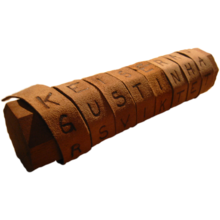
\includegraphics[width=5cm]{img/scitala.png} }}%
%    %\caption{2 Figures side by side}%
%    %\label{fig:example}%
%  \end{figure}
%
%\end{frame}
%
%\begin{frame}{{Cryptography today}
%  \center {
%    Le necessità, così come le risorse a disposizione, si sono evolute 
%    
%    ed oggi possiamo suddividere la crittografia in:
%     
%    \pause
%    
%    \medskip
%    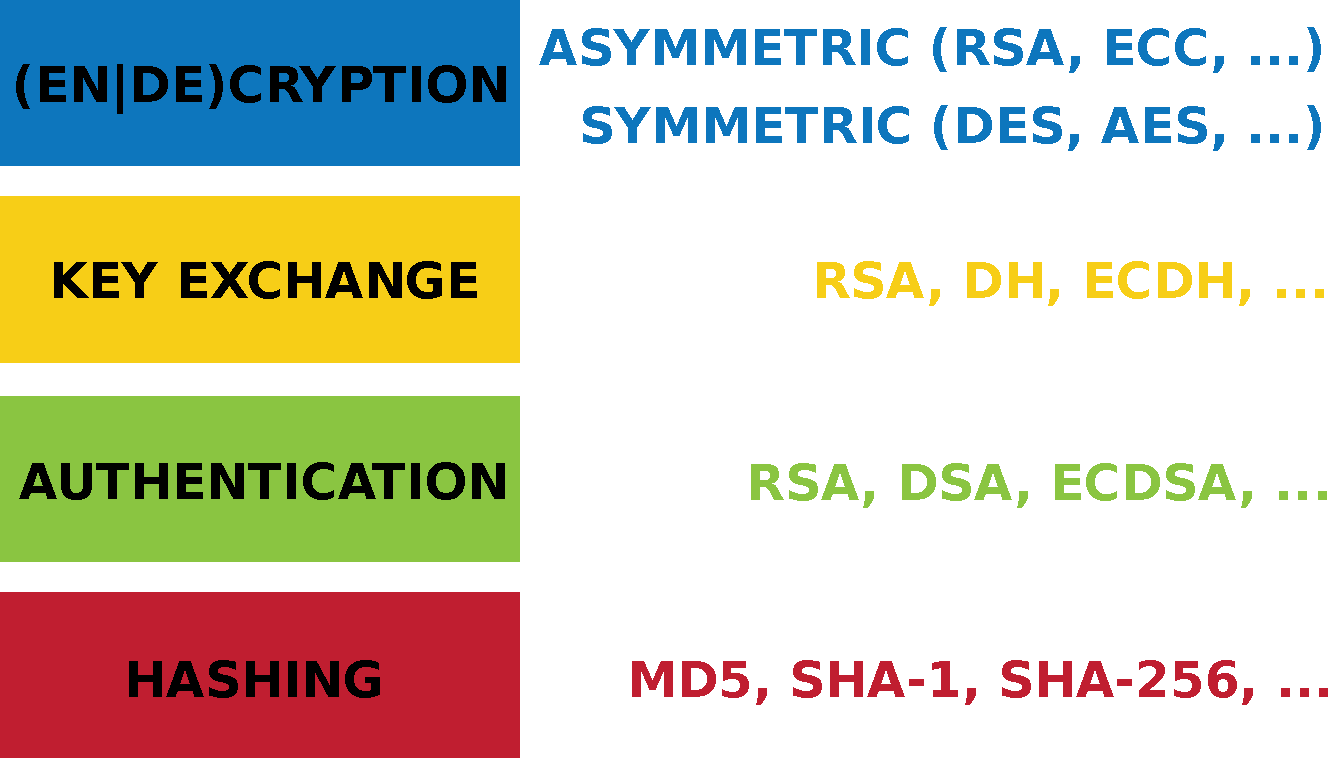
\includegraphics[width=0.6\textwidth]{include/crypto-section.pdf}
%  }
%\end{frame}
